\newpage \section{The npde package} \label{sec:progdesc}

\subsection{Preparation of the input}

\hskip 18pt The library needs two files: 
\begin{itemize} 
\item the file containing the dataset to be evaluated (hereafter named 'observed data') \item the file containing 
the simulations (hereafter named 'simulated data') 
\end{itemize} 
The library does not perform the simulations. {\sf R}, {\sf NONMEM}~\cite{NONMEM}, {\sf 
MONOLIX}~\cite{Monolix} or any program of your choice can be used for that purpose.

\subsubsection{Observed data}

\hskip 18pt The observed data file must contain at least the following 3 columns: 
\begin{itemize} 
\item id: patient identification 
\item xobs: independent variable (time, X, ...) 
\item yobs: dependent variable (DV, concentrations, 
effects...) 
\end{itemize} 
Additional (optional) columns may be given. The program will recognise the following 
input: 
\begin{itemize} 
\item cens: censoring information (0 for observed data, 1 for censored data) 
\item mdv: missing data (0 for observed data, 1 for missing data); this information supersedes censoring 
information, so that an observation with mdv equal to 1 will be treated as missing, not as censored; observations 
with values "." or NA will also be considered as missing 
\item ipred: individual model predictions 
\item covariates 
\end{itemize} 
The computation of \pd~and \npde~will remove missing observations from the observed dataset reported in the output 
(see section~\ref{sec:results}). If other names than {\sf cens} and {\sf mdv} are used in the original dataset, 
they will be renamed to {\sf cens} and {\sf mdv} in the {\sf data} slot of the object.

Other columns may be present but will not be used by the library. The actual order of the columns is unimportant, 
since the user may specify which column contain the requested information, but the default order is 1. id, 2. xobs, 
3. yobs and no MDV column. A file header may be present, and column separators should be one of: blank space(s), 
tabulation mark, comma (,) or semi-colon (;). Finally, the digit mark should be a dot as in English (eg a number 
would read 4.5) and not a comma as in French (4,5).

\subsubsection{Simulated data}

\hskip 18pt The user must provide a file containing the K simulated datasets stacked one after the other. Within 
each simulated dataset, the order of the observations must be the same as within the observed dataset. The 
dimensions of the two datasets must be compatible: if n$_{\rm obs}$ is the number of lines in the observed dataset, 
the file containing the simulated datasets must have K$\times$n$_{\rm obs}$ lines.

The simulated data file must contain at least 3 columns, in the following order: \begin{enumerate} \item id : 
patient identification \item xsim: independent variable (time, X, ...) \item ysim: dependent variable (DV, 
concentrations, effects...) \end{enumerate} Additional columns may be present but will not be used by the library.

The length of the \textcolor{violet}{id} (resp \textcolor{violet}{xobs}) column must be equal to the length of the 
\textcolor{violet}{id} (resp \textcolor{violet}{xobs}) column of the observed dataset repeated K times.

An example of how to set up simulations for an example dataset can be found in section~\ref{sec:exampletheo}, and 
examples of a simulated and observed dataset are available in the subdirectory {\sf doc/inst} of the library.

\subsubsection{Number of simulations}

\hskip 18pt Based on the results of simulation studies~\cite{Brendel10,Comets10}, we recommend to use at least 
$K$=1000 but the actual number may depend on the dataset involved, and should be increased when the dataset 
includes a large number of subjects. This will be investigated in more details in future work on {\sf npde}. A 
warning will be issued when $K$ is smaller than 1000 (see examples in section~\ref{sec:npde.examples}).

\subsection{Execution}

\subsubsection{Interactive execution}

\hskip 18pt The interactive mode is called by the function {\sf npde()}: 
\begin{verbatim} 
myres<-npde() 
\end{verbatim} 
The user will be prompted to enter successively: 
\begin{itemize} \item the name of the file or dataframe containing the observed data 
\item the columns in which id, xobs, dependent variable yobs, and possibly 
column with missing data MDV can be found (the default order is 1, 2, 3 and no MDV column) \item the name of the 
file or dataframe containing the simulated data 
\item whether results should be saved to disk; if so, the user must also enter 
    \begin{itemize} 
    \item the format of the graph (one of: Postscript, JPEG, PNG or PDF) 
    \item the name of the files: an extension {\sf .npde} will be added to this name for the file in which 
numerical     results are to be saved (see section~\ref{sec:results}), and an extension depending on the format of 
the graph will     be added to this name for the file in which graphs are to be saved (respectively .eps, .jpeg, 
.png, .pdf for the     formats above). For instance, if the user enters {\sf myoutput} and requests that the graphs 
be saved in PDF     format, the results file will be named {\sf myoutput.npde} and the graph files will be {\sf 
myoutput.pdf}. 
    \end{itemize} 
\item whether $\npde$ should be computed \item whether $\pd$ should be computed \item whether a message should be 
printed as the computation of $\npde$ begins in a new subject 
\item whether the function should return values (see section~\ref{sec:value}) 
\end{itemize} 
Alternatively, one or both filenames for the observed and simulated data 
can be replaced by a dataframe if the data has already been loaded in {\sf R} (see example in the online 
documentation provided with the package).

\subsubsection{Non-interactive execution}

\hskip 18pt In the non-interactive mode, the required information is fed to the function {\sf autonpde()} instead 
of answering a series of questions. The minimum input should include the name of the observed data file (for 
example, {\sf theopp.tab}) and the name of the simulated data file (for example, {\sf simtheopp.tab}), as in: 
\begin{verbatim} autonpde("theopp.tab","simtheopp.tab") \end{verbatim} A number of options can also be set as 
arguments, and are given in table~I. \begin{table}[!h] \noindent{\bfseries Table I:} {\itshape Options available 
for the autonpde function.} \begin{center} \begin{tabular} {l p{8cm} c} \hline \textbf{Option} & \textbf{Effect} & 
\textbf{Default value} \\ \hline iid & number of the column with ID information in the observed data file & 1 \\ ix 
& number of the column with the independent variable (X) & 2 \\ iy & number of the column with the observed data 
(Y) & 3 \\ imdv & number of the column indicating missing data (MDV) & 0 \\ icens & number of the column indicating 
censoring (CENS) & 0 \\ iipred & number of the column with individual predictions (IPRED) & 0 \\ detect & if TRUE, 
the datafile containing the original data is assumed to have a header, and the program will attempt to guess which 
columns contain ID, X, Y, MDV, CENS and IPRED & FALSE \\ units & units for the X and Y axis (will be used in plots) 
& none \\ boolsave & whether results should be saved to disk & TRUE \\ namsav & name of the files where results 
will be saved (without extension) & output\\ type.graph & graph format (one of: Postscript, JPEG, PNG or PDF, 
corresponding to extensions .eps, .jpeg, .png and .pdf respectively for the graph file) & eps \\ calc.npde & 
whether normalised prediction distribution errors should be computed &  TRUE \\ calc.pd & whether prediction 
discrepancies should be computed & TRUE \\ decorr.method & method used to decorrelate & cholesky \\ cens.method & 
method used to handle censored data & impute \\ ties & if FALSE, the distributions of \pd and \npde are smoothed to 
avoid ties & TRUE \\ verbose & whether a message should be printed as the computation of $\npde$ begins in a new 
subject &  FALSE \\ \hline \end{tabular} \end{center} \end{table} Note that option \texttt{output} has been 
deprecated (the \texttt{invisible()} option is used to suppress the output when it is not affected to an object).

\bigskip Here is an example of the call to {\sf autonpde()} with a number of arguments (see example in 
section~\ref{sec:expde} for an illustration): \begin{verbatim} 
x<-autonpde(namobs="theopp.tab",namsim="simtheopp.tab",iid=1,ix=2,iy=3, 
imdv=0,namsav="output.eps",boolsave=T,type.graph="eps",output=F,verbose=T) \end{verbatim}

\clearpage \subsection{Results} \label{sec:results}

\hskip 18pt Both execution modes will produce the same results. Three types of results are produced by default, but 
options can be used so that only some of them are created: \begin{enumerate} \item an {\sf R} object of class 
NpdeObject, containing several elements, including the $\npde$ and/or $\pd$ (see section~\ref{sec:value}). With the 
option {\sf output=F} the object is not returned. \item a graph file containing diagnostic plots of the $\npde$ 
({\sf output.eps} with the default values; see section~\ref{sec:graphics}). The graph also appears in the graphic 
window of the current {\sf R} session. With the option {\sf boolsave=F} the graph is shown but not saved to a file. 
\item a text file with the same name as the graph file and extension {\sf .npde} containing the following data 
({\sf output.npde} with the default values), organised in columns: id, xobs, ypred, npde, pd With the option {\sf 
boolsave=F}, the results are not saved. \end{enumerate}

\subsubsection{Value}~\label{sec:value}

\hskip 18pt By default, the function returns an object of class NpdeObject: \begin{verbatim} myres<-npde() 
\end{verbatim} Version 2.0 of the \npde~package uses the S4 class system, and many functions have been defined to 
handle the object and produce descriptive summaries and plots (please refer to section~\ref{sec:npde.methods} for 
more details about S4 classes). As a result, the output is no longer a list that can be manipulated, but a slightly 
more complicated object. However, for compatibility with the previous version of \npde, a \texttt{summary} function 
can be used to produce a list containing the main results: \begin{verbatim} x1<-summary(myres) \end{verbatim}

\bigskip The object returned by the function contains 5 elements: \begin{enumerate} \item \textbf{data}: a NpdeData 
object containing the information relative to the observed data \item \textbf{datsim}: a NpdeSimData object 
containing the information relative to the simulated data \item \textbf{results}: a NpdeRes object containing the 
results \item \textbf{options}: a list of options used in the computations \item \textbf{prefs}: a list of 
graphical preferences \end{enumerate} The first three elements are S4 objects also, with their own class and own 
methods, while the last two elements are R lists. More information on how to handle these objects and which methods 
have been defined for them can be found in~\ref{sec:npde.methods}.

\subsubsection{Graphs} \label{sec:graphics}

\hskip 18pt Four graphs are produced by default: \begin{enumerate} \item a quantile-quantile plot: plot of the 
$\npde$ versus the corresponding quantiles of a normal distribution \begin{itemize} \item the line $y=x$ is also 
drawn \end{itemize} \item a histogram of the $\npde$ \begin{itemize} \item the shape of the normal distribution 
$\mathcal{N}(0,1)$ is also shown \end{itemize} \item a plot of the $\npde$ versus the independent variable X \item 
a plot of the $\npde$ versus ypred \begin{itemize} \item for these last two graphs, we plot the lines corresponding 
to $y=0$ and to the critical values 5\% and 95\% (delimiting the 90\% confidence interval in which we expect to 
find the bulk of the $\npde$). \end{itemize}   \end{enumerate} The default graphs now include (approximated) 
prediction intervals (obtained by simulating from the theoretical $\mathcal{N}(0,1)$ distribution, see 
section~\ref{sec:graphmethods}); for compatibility with the behaviour of \npde~version 1.2, the option {\sf 
bands=FALSE} can be used to suppress plotting the prediction intervals.

These graphs are designed as diagnostics for the $\npde$; a function providing similar graphs for $\pd$ is {\sf 
plotpd}.

\subsection{Errors during execution}

\hskip 18pt Sometimes the function is unable to compute the decorrelated prediction distribution errors for one or 
more subjects. The following error messages can appear: \begin{verbatim} The computation of the npde has failed for 
subject xx because the Cholesky decomposition of the covariance matrix of the simulated data could not be obtained. 
\end{verbatim} or \begin{verbatim} The computation of the npde has failed for subject xx because the covariance 
matrix of the simulated data could not be inverted. \end{verbatim} followed by: \begin{verbatim} This usually means 
that the covariance matrix is not positive-definite. This can be caused by simulations widely different from 
observations (in other words, a poor model). We suggest to plot a prediction interval from the simulated data to 
check whether the simulations are reasonable, and to consider prediction discrepancies. Prediction discrepancies 
will now be computed. \end{verbatim} In our experience, this usually happens when the model is so ill-conditioned 
that the matrices involved in the computation of the prediction distribution errors are singular, and mostly 
happens when the model predicts the data very poorly. A prediction interval (or Visual Predictive Check) can be 
plotted to check this.

When $\npde$ cannot be computed, the program computes automatically $\pd$ even if the {\sf calc.pd=F} option was 
used. The following graphs are plotted using $\pd$ instead of $\npde$ \begin{enumerate} \item a quantile-quantile 
plot: plot of the $\pd$ versus the corresponding quantiles of a uniform distribution \begin{itemize} \item the line 
$y=x$ is also drawn \end{itemize} \item a histogram of the $\pd$ with the uniform density $\mathcal{U}(0,1)$ 
overlain \item a plot of the $\pd$ versus the independent variable X \item a plot of the $\pd$ versus $\ypred$ 
\begin{itemize} \item for these last two graphs, we plot the lines corresponding to $y=0$ and to the 5\% and 95\% 
critical values (delimiting the 90\% confidence interval in which we expect to find the bulk of the $\pd$). 
\end{itemize} \end{enumerate} In this case, approximated prediction intervals are not plotted by default, since the 
approximation (sampling from the standard gaussian distribution) neglects the correlation between the different 
$\pd$ in an individual, and this leads to substantially narrower prediction intervals when the number of data per 
subject is large. Prediction bands may be added by combining the option {\sf bands=TRUE} with option {\sf 
approx.pi} set to either \texttt{TRUE} for an approximated prediction interval (fast but rough) or \texttt{FALSE} 
for an approximated prediction interval (obtained using the simulated datasets), as in: \begin{verbatim} 
x<-dist.pred.sim(x) plot(x,bands=TRUE,approx.pi=TRUE) \end{verbatim} As seen here, requesting an exact (simulated) 
prediction interval requires first to compute the distribution of $\pd$ in the simulated dataset, using the 
function \texttt{dist.pred.sim} (by default and in the interest of time, this function computes only the 
distribution of the $\pd$, but if called with the additional argument {\sf calc.npde=TRUE} the $\npde$ in the 
simulated dataset will also be included in the output, allowing the user to use \texttt{approx.pi=TRUE} for graphs 
including $\npde$).

\subsection{Functions in the \npde~package} \label{sec:npde.methods}

\hskip 18pt \npde~has been programmed using the S4 classes in \R. S4 classes implement Object oriented programming 
(OOP) in \R, allowing to construct modular pieces of code which can be used as black boxes for large systems. Most 
packages in the base library and many contributed packages use the former class system, called S3. However, S4 
classes are a more traditional and complete object oriented system including type checking and multiple 
dispatching. S4 is implemented in the methods package in base \R. More information on S4 classes and \R packages 
can be found in tutorials on the Web. I used extensively the following manual~\cite{Genolini} (in French).

The object returned by the \texttt{npde()} and \texttt{autonpde()} functions has the \texttt{NpdeObject} class, and 
both generic and specific methods have been defined for this class: \begin{itemize} \item print: the print function 
produces a summary of the object in a nice format \item show: this function is used invisibly by \R when the name 
of the object is typed, and produces a short summary of the object (more details can be obtained by using the 
alternative \texttt{showall()} function \item summary: this function produces a summary of the object, and 
invisibly returns a list with a number of elements, which provides an alternative way to access elements of the 
class; the list contains the following elements: \begin{itemize} \item[obsdat] the data (a matrix with 3 columns, 
id=subject id, xobs=observed X, yobs=observed Y, plus if present in the data additional columns containing censored 
information, mdv, covariates, ...) \item[id] subject id (first column in obsdat) \item[x] observed x (second column 
in obsdat) \item[y] observed y (third column in obsdat) \item[npde] the computed $\npde$ \item[pd] the computed 
prediction discrepancies \item[ploq] the probability of being BQL for each observation (if computed) \item[N] 
number of subjects \item[nrep] number of simulations used in the computations \item[ntot.obs] total number of 
non-missing observations \item[ypred] predicted Y (the empirical mean of the simulated predicted distribution for 
each observation ($E_k(y^{sim(k)}_{ij})$)) \item[ycomp] completed vector of observed y (includes the values that 
were imputed during the computation when BQL data are in the dataset) \item[ydobs] the decorrelated observed data 
$y_{ij}^*$ \item[ydsim] the decorrelated simulated data $y^{sim(k)*}_{ij}$ \item[xerr] an integer valued 0 if no 
error occurred during the computation or a positive number (1 or 2) depending on the error encountered, if an error 
occurred \item[options] options (can also be seen by using the \texttt{print} function) \item[prefs] graphical 
preferences (can also be seen by using the \texttt{print} function) \end{itemize} \item plot: this produces plots 
of the different objects \begin{itemize} \item when called without any argument, the default four plots are 
produced \item an argument plot.type can be used to produce different plots \item all plots can be tweaked to add 
titles, change colours,... \end{itemize} \item $[$ function: the get function, used to access the value of the 
slots in an object \item $[<$-: function: the set function, used to replace the value of the slots in an object 
\item gof.test: goodness-of-fit tests on the distribution of \texttt{npde} (or \texttt{pd}) \end{itemize} Examples 
of calls to these functions are given in the corresponding man pages and in the documentation 
(section~\ref{sec:exampletheo}).

\subsection{Options for graphs}

\hskip 18pt The document \verb+ test_npde.pdf+ has been created to test the \npde~library and showcase the 
different graphs. It contains several fits for the datasets shown in section~\ref{sec:npde.examples}, and provides 
many examples of graphs setting graphical options. There is also a list of the graphical options with their 
significance. This document is included in the \verb+inst+ directory, where the present guide is also located.

\bigskip An object \texttt{x} resulting from a call to {\sf npde()} or {\sf autonpde()} contains a slot 
\texttt{prefs} where the graphical preferences are stored as a list. Options can be set on the fly for a given 
plot, by simply adding them to the call to {\sf plot()} as an argument (see examples in 
section~\ref{sec:npde.examples}), and they will then supersede the preferences attached to the object: 
\begin{verbatim} plot(x,plot.type="data",col="red",main="Raw data") \end{verbatim} The options can also be modified 
directly in the object, and they will then apply to the next plots, for instance changing the new default color to 
red for all plots is done by setting the attribute {\sf col} in the list: \begin{verbatim} x["prefs"]$col<-"red" 
\end{verbatim} Options given on the fly will always supersede the options stored in the \texttt{prefs} slot.

\paragraph{Binning:} most graphs now have the option of added prediction intervals. These prediction intervals are 
computed using simulations under the model, and they require a binning algorithm. The influence of the number and 
position of bins is quite important for the visual assessment of the fit.

Several options are available for binning, and can be set using the \texttt{vpc.method} option. Possible options 
are: \begin{itemize} \item \texttt{equal}: uses quantiles of the data to have about the same number of points in 
each bin \item \texttt{width}: divides the interval into bins of equal size \item \texttt{user}: user-defined 
breakpoints, set in \texttt{vpc.breaks} (will automatically be expanded to include the lower and upper value of the 
data if not provided) (if \texttt{vpc.breaks} is not supplied, the \texttt{equal} method will be used instead) 
\item \texttt{optimal}: uses the \texttt{Mclust} function from the \texttt{mclust} library (when available) to 
provide the optimal clustering; the Mclust method \end{itemize} With all methods, if the number of bins requested 
is larger than the number of unique values of X, the number of bins will be limited to the number of unique values.

\begin{description} 
\item[Warning:] when using the 'optimal' method, warnings may appear. The optimal number of bins is selected from 
a range equal to \texttt{vpc.bin} $\pm 5$, but a message such as:
'\verb+In map(out$z) : no assignment to 2,4,8,11+' usually indicates that the number of bins is too large, it is 
then advised to change the value of \texttt{vpc.bin} and start again. 
\end{description}

Specifying c(0.01,0.99) with the '\texttt{equal}' or '\texttt{width}' binning method and vpc.bin=10 will create 2 
extreme bands containing 1\% of the data on the X-interval, then divide the region within the two bands into the 
remaining 8 intervals each containing the same number of data; in this case the intervals will all be equal except 
for the two extreme intervals, the size of which is fixed by the user; complete fine-tuning can be obtained by 
setting the breaks with the vpc.method="user"

\paragraph{Further options:} More details on available graphs and options can be found in the online documentation. 
Please type: 
\begin{verbatim} 
?plot.npde 
\end{verbatim} to get started. 
% The npde library contains 14 functions. Figure~\ref{fig:functionhierar} presents 
% the functions hierarchy starting with function {\sf npde}. A similar graph is 
% obtained with function {\sf autonpde} without the call to function {\sf % pdemenu}. 
% \begin{figure}[!h] %\begin{center} 
% 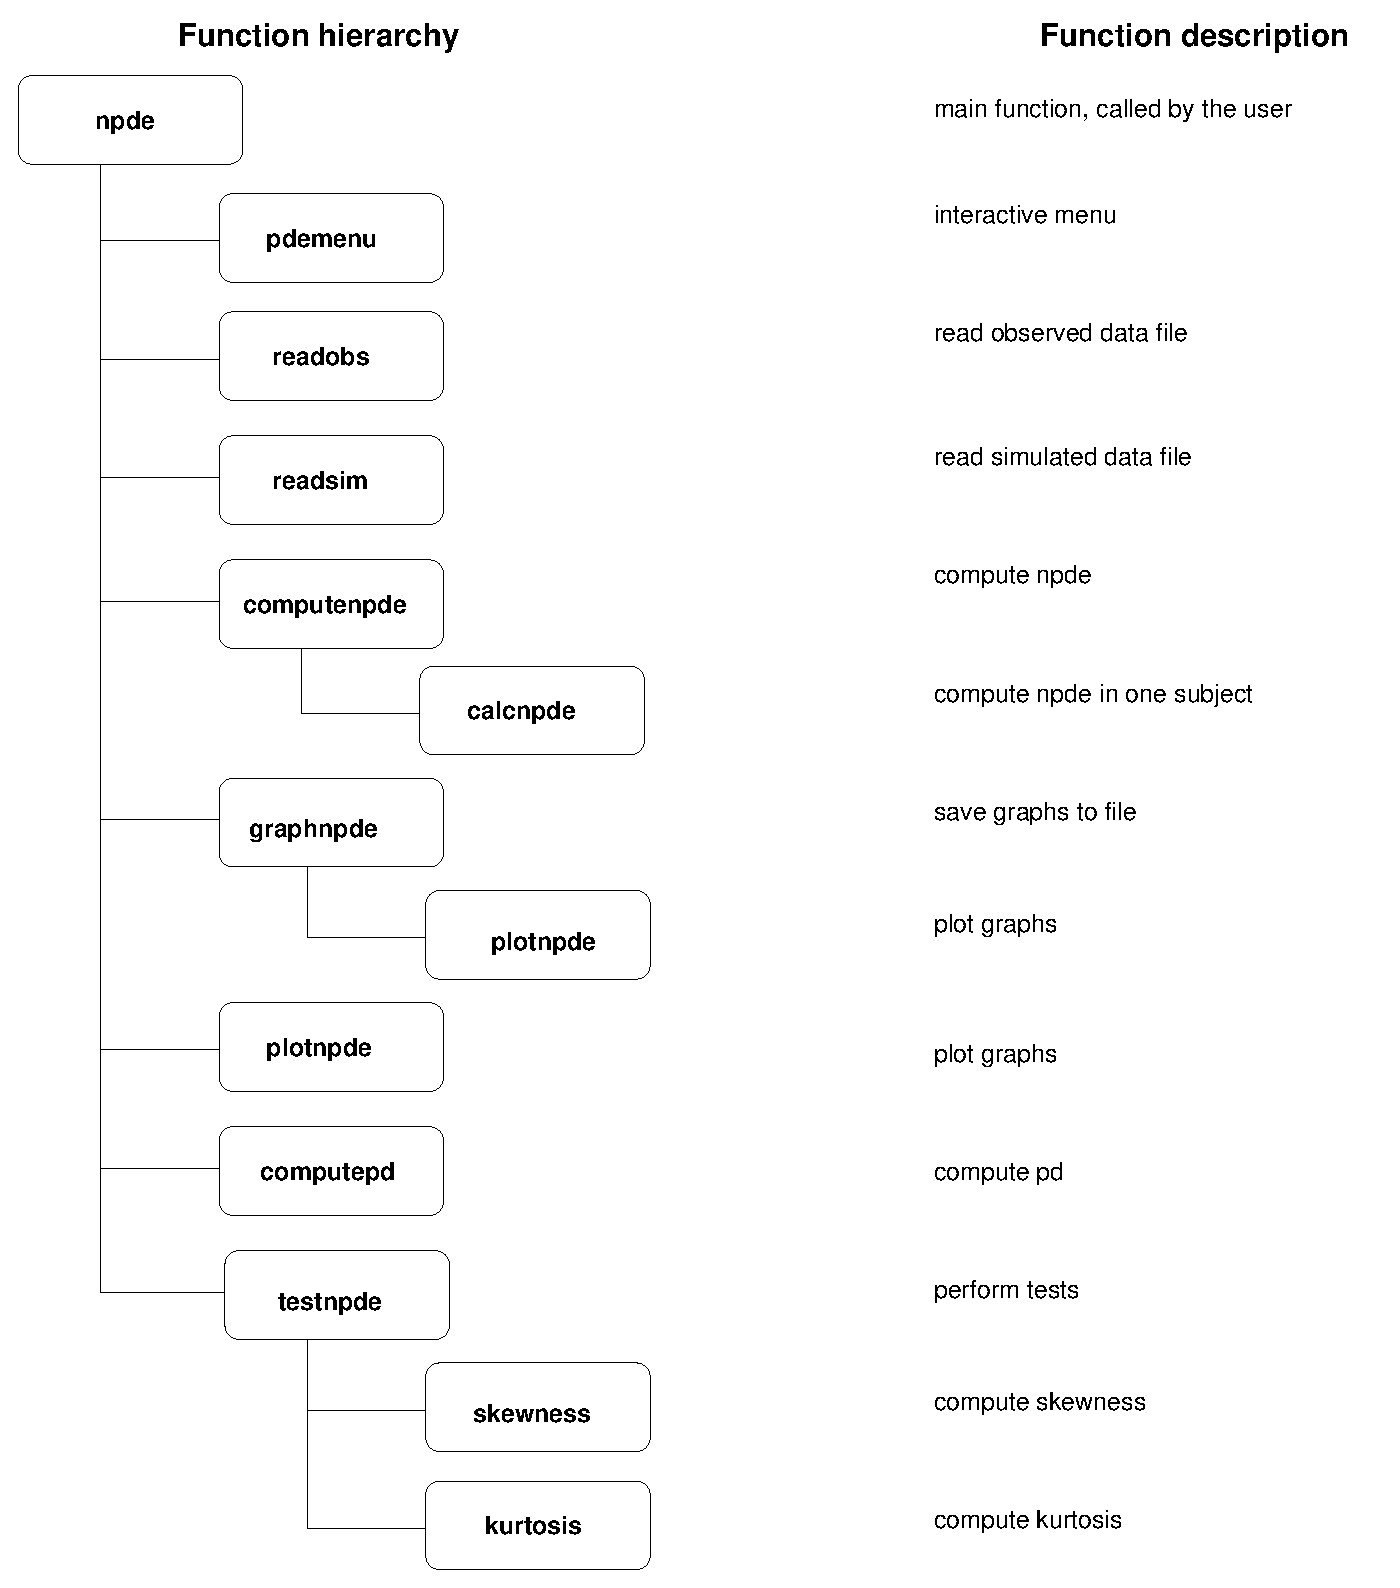
\epsfig{file=/home/eco/work/npde/doclib/figs/hierarchyhelv.eps,width=16cm,angle=0} % \end{center} 
% \par \kern -1cm 
% \caption{Function hierarchy for the npde package, and brief description of each 
% function. The functional hierarchy is given for a user call to npde. With 
% autonpde, the hierarchy is the same save for the initial call to pdemenu.} 
% \label{fig:functionhierar} 
% \end{figure}

If further tweaking is required, any graph can also be recreated with a bit of work using the output from the 
package. Using the function \texttt{summary} will extract the necessary elements from the object, and the user can 
then use those to produce her or his own graphs. \begin{verbatim} x1<-summary(x) names(x1) head(x1$x) head(x1$npde) 
\end{verbatim}

\clearpage \newpage
